    \section{Regulator PID} 
    
    \subsection{Implementacja}
         Najważniejszą częścią programu jest implementacja regulatora PID. Odpowiednie zaprojektowanie jego działania jest kluczowe w kwestii wydajności oraz poprawności funkcjonowania całego systemu. Schemat funkcjonowania algorytmu jest prosty. Został on przedstawiony na listingu \ref{code:pid_compute}. 
         
         Czytamy ilość impulsów z układu odpowiedzialnego za ich zliczanie. Przy okazji czyścimy jego rejestry, aby mógł zliczać już kolejne impulsy w trakcie, gdy my będziemy dokonywać obliczeń. Realizacja tego jest przesłonięta przez marko zawarte w \ref{code:encoder_macro} w celu zwiększenia czytelności kodu. 
         
        \begin{kod}
          \inputminted[firstline=10,lastline=12]{cpp}{esp/listings/encoder_driver.hpp}
          \caption{Pobieranie wartości i czyszczenie rejestrów licznika}
          \label{code:encoder_macro}
          \vspace{1em}
        \end{kod}
         
         
         Warto zaznaczyć że nie zapisujemy momentu zaczytania danych. Musimy więc zagwarantować że funkcja ta będzie wykonywać się cyklicznie w ściśle określonym przedziale czasowym. Każde odstępstwo od tego będzie powodowało błędy w poprawnym działaniu algorytmu. 
         
        \begin{kod}
          \inputminted[firstline=17,lastline=45]{cpp}{esp/listings/pid.cpp}
          \caption{Pętla regulatora PID}
          \label{code:pid_compute}
          \vspace{2em}
        \end{kod}
    
         Kolejnym krokiem jest policzenie uchybu regulacji. Jest to tradycyjnie różnica wartości ustalonej i zliczonych impulsów. Następnie liczymy wartości dla każdego z członów regulacji, jednocześnie gwarantując że mieszczą się one we wcześniej zdefiniowanych przedziałach. To również ukryte zostało pod makrem dostępnym w listingu \ref{code:pid_macro}.
         
         Wartości każdego z członów mnożymy poprzez wybrane przez użytkownika współczynniki. Są one zapisane w zmiennych dzięki czemu istnieje możliwość zmiany ich wartości dynamicznie podczas pracy programu. Teraz wystarczy już zsumować wszystkie wartości oraz zapewnić że uzyskana wartość nie przekroczy wartości granicznych możliwych do ustawienia dla PWM. W tym momencie część obliczeniowa jest gotowa. Istnieje jednak spore ryzyko że uzyskana w ten sposób wartość nie będzie mieściła się w zakresie przyjmowanym przez peryferium odpowiedzialnym za modulowanie napięcia. Niezbędne jest więc wykonanie kolejnej normalizacji do akceptowalnych wartości  \ref{code:pid_macro}. 
       
        \begin{kod}
          \inputminted[firstline=10,lastline=16]{cpp}{esp/listings/pid.hpp}
          \caption{Normalizacja wartości regulatora}
          \label{code:pid_macro}
          \vspace{1em}
        \end{kod}
    
    \subsection{Proces PID}
        Pętla regulatora PID zaimplementowana jest w swoim własnym procesie. Ułatwia to kontrolę częstości wykonywania obliczeń i umożliwia zatrzymanie procesu gdy jest on niepotrzebny. Na przykład przy braku połączenia z serwerem MQTT.
        
        Implementacja procesu zawarta jest w listingu \ref{code:pid_task}. Pierwsze linie kodu rozpoczynają inicjalizację niezbędnych obiektów. W skład nich wchodzi:
        
        \begin{itemize}
            \item config - struktura zawierająca konfigurację parametrów regulatora. Niezbędna do dynamicznej zmiany parametrów PID.
            
            \item engine - instancja sterująca peryferium PWM,
            \item encoder - instancja do obsługi enkodera,
            \item pid - instancja regualtora PID,
            \item pid\_result - zmienna zawirająca wyliczoną wartość regulacji,
        \end{itemize}
        
        Kolejne linie kodu wykonują się w nieskończonej pętli. Następuje w niej odczyt aktualnego stanu licznika systemowego. Jest on wykorzystywany do wyliczenia jak długo wykonują się operacje w pętli. Następnie sprawdzana jest kolejka FIFO. W przypadku znalezienia się w niej nowej konfiguracji dla regulatora, jest ona natychmiast zastosowana. 
        
        \begin{kod}
          \inputminted[firstline=58]{cpp}{esp/listings/pid.cpp}
          \caption{Proces wykonywanie PID}
          \label{code:pid_task}
          \vspace{2em}
        \end{kod}
        
        Po opuszczeniu instrukcji warunkowej następuje obliczenie wartości regulatora i ustawienie modulacji szerokości impulsu zgodnie z uzyskanym wynikiem. Ostatnim krokiem jest zatrzymanie procesu. Czas zatrzymania jest zależny od prędkości wykonywania pętli i warunkuje częstotliwość wyzwalania PID na 100Hz. Na obrazku \ref{fig:pid_plantuml} znajduje się diagram aktywności opisywanego procesu.
        
                      
        \begin{figure}[ht]
            \centering
            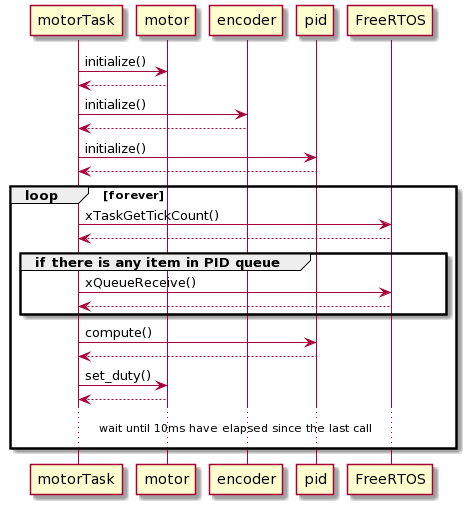
\includegraphics[width=0.8\textwidth]{img/motorTask_uml.png}
            \caption{Diagram aktywności procesu PID}
            \label{fig:pid_plantuml}
        \end{figure}